\section{Results and Discussion}

The longitudinal and transversal spatial wave function densities for $\eta = 23 \, \omega_\text{r}$ are depicted in Figure~\ref{densities}. The first two states are degenerate states. Both for longitudinal and transversal pump, because of equal contributions of $a$ and $a^\dagger$, the spatial densities are $\lambda / 2$-periodic.

\begin{figure}[!htb]
	\begin{minipage}[b]{1\linewidth}
	\centering
	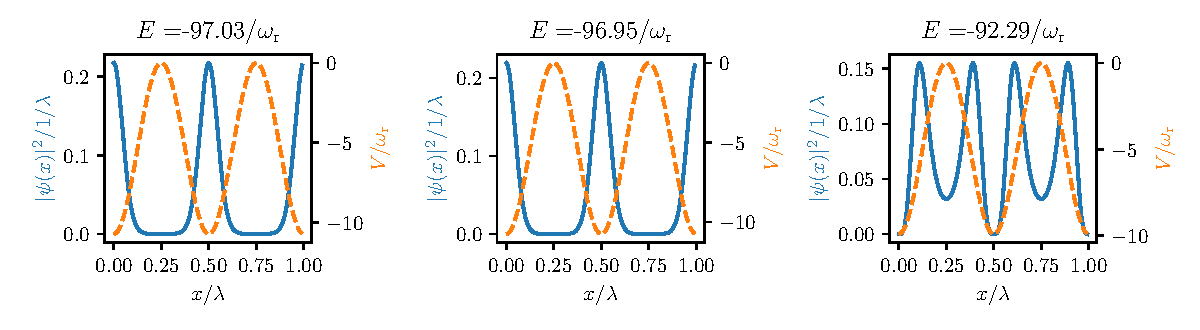
\includegraphics[width=1\textwidth]{images/dens_long.pdf}
	\subcaption{Longitudinal.}
	\label{long_density}
	\end{minipage}
%
	\begin{minipage}[b]{1\linewidth}
	\centering
	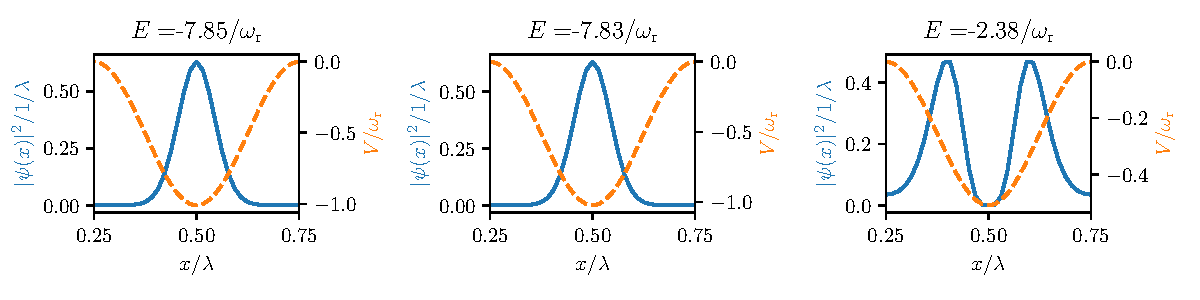
\includegraphics[width=1\textwidth]{images/dens_trans.pdf}
	\subcaption{Transversal.}
	\label{trans_density}
	\end{minipage}
\caption{Longitudinal and transversal wave function densities for $\eta = 60 \omega_\text{r}$.}
\label{densities}
\end{figure}
\FloatBarrier

\noindent The momentum distribution for different values of $\eta$ can be seen in Figure~\ref{momenta}. The transversal pump doesn't peak as high as the longitudinal pump. Between every bar there's a gap in the longitudinal pump. The bigger we set $\eta$, the wider becomes the distribution.

\begin{figure}[!htb]
	\begin{minipage}[b]{1\linewidth}
	\centering
	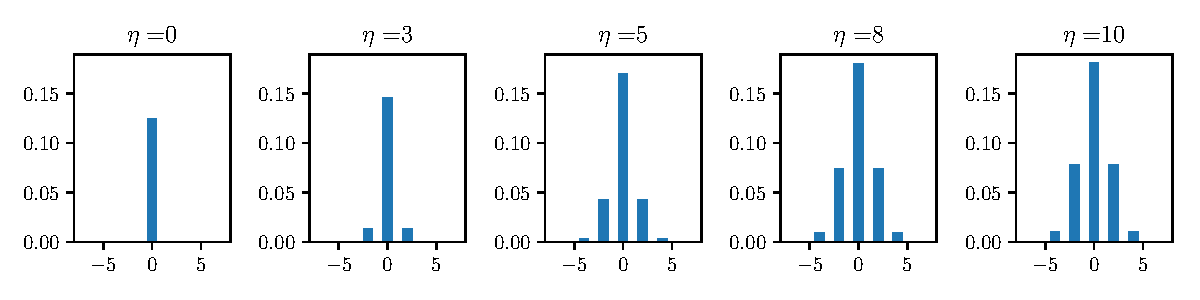
\includegraphics[width=1\textwidth]{images/mom_long.pdf}
	\subcaption{Longitudinal.}
	\label{long_momentum}
	\end{minipage}
%
	\begin{minipage}[b]{1\linewidth}
	\centering
	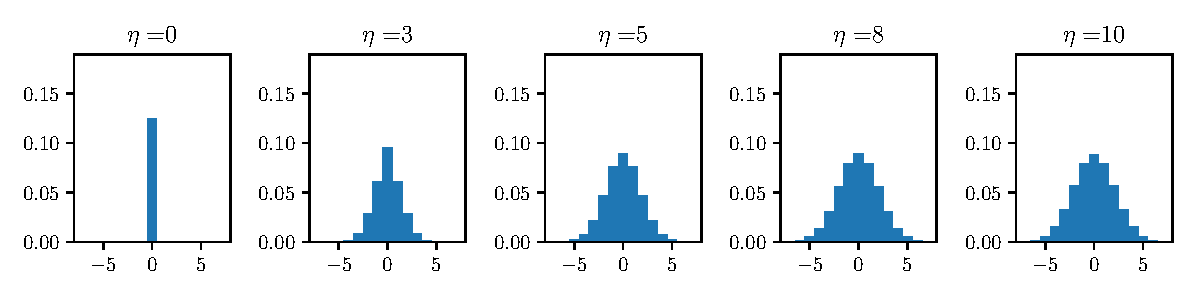
\includegraphics[width=1\textwidth]{images/mom_trans.pdf}
	\subcaption{Transversal.}
	\label{trans_momentum}
	\end{minipage}
\caption{Longitudinal and transversal momentum distributions.}
\label{momenta}
\end{figure}
\FloatBarrier

\noindent The photon number distribution for different values of $\eta$ can be seen in Figure~\ref{photon_dist}. Initially, it looks like a Poisson distribution, but this is less and less the case for higher values of $\eta$. For a Poisson distribution, the mean and the variance have to be the same.

\begin{figure}[!htb]
	\begin{minipage}[b]{1\linewidth}
	\centering
	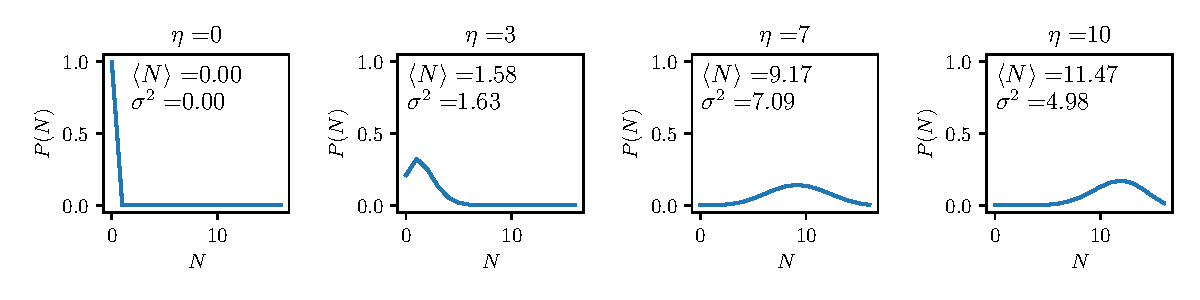
\includegraphics[width=1\textwidth]{images/pho_dens_long.pdf}
	\subcaption{Longitudinal.}
	\end{minipage}
%
	\begin{minipage}[b]{1\linewidth}
	\centering
	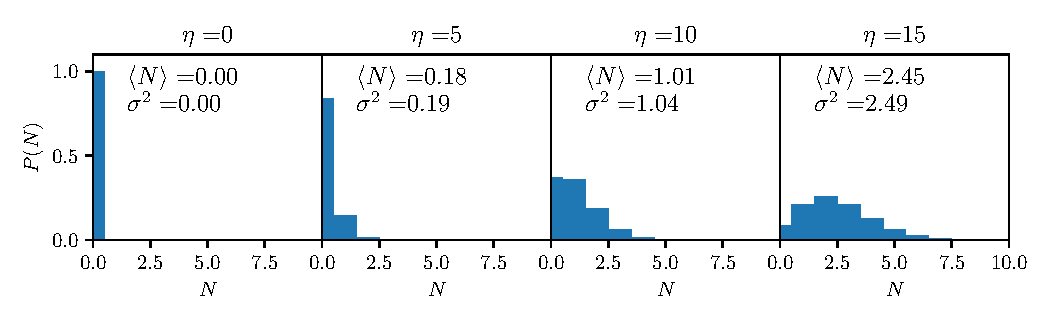
\includegraphics[width=1\textwidth]{images/pho_dens_trans.pdf}
	\subcaption{Transversal.}
	\end{minipage}
\caption{Longitudinal and transversal photon distributions.}
\label{photon_dist}
\end{figure}
\FloatBarrier

\noindent The Husimi Q representation of both longitudinal and transversal pump can be seen in Figure~\ref{qfunc}.

\begin{figure}[!htb]
	\begin{minipage}[b]{1\linewidth}
	\centering
	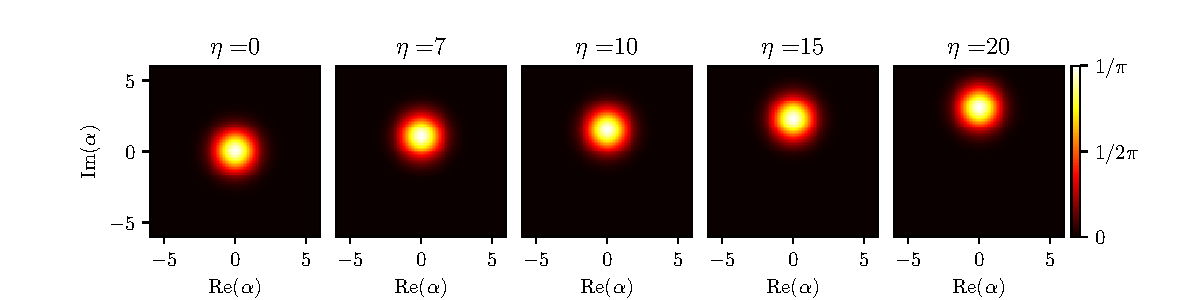
\includegraphics[width=1\textwidth]{images/qfunc_long.pdf}
	\subcaption{Longitudinal.}
	\end{minipage}
%
	\begin{minipage}[b]{1\linewidth}
	\centering
	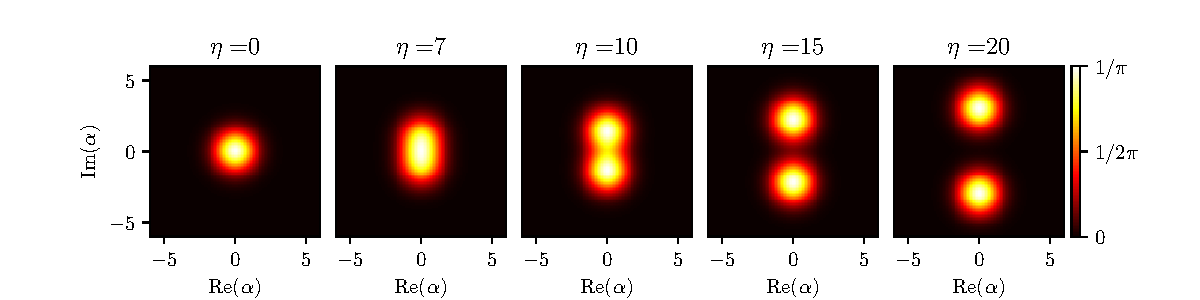
\includegraphics[width=1\textwidth]{images/qfunc_trans.pdf}
	\subcaption{Transversal.}
	\end{minipage}
\caption{Husimi Q representation of longitudinal and transversal wave functions.}
\label{qfunc}
\end{figure}
\FloatBarrier

\noindent The order parameter $\Theta$ can be seen in Figure~\ref{fig_order_param}. For longitudinal pumping, there's no threshold at which order sets in rapidly, but a linear increase. For transversal pumping, we can clearly observe such a threshold.

\begin{figure}[!htb]
	\begin{minipage}[b]{.5\linewidth}
	\centering
	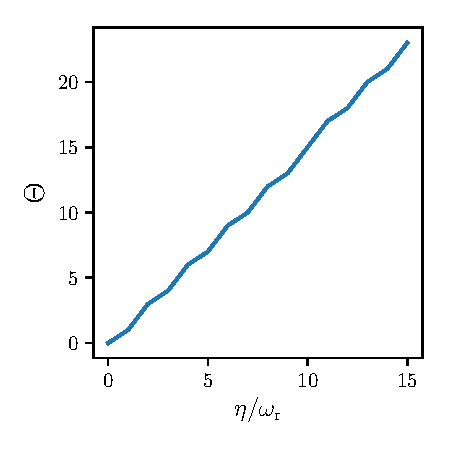
\includegraphics[width=.9\textwidth]{images/theta_long.pdf}
	\subcaption{Longitudinal.}
	\end{minipage}
%
	\begin{minipage}[b]{.5\linewidth}
	\centering
	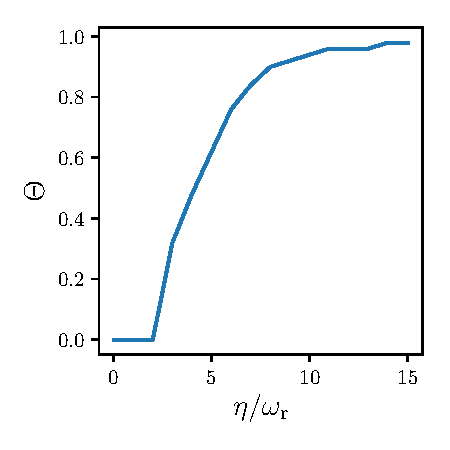
\includegraphics[width=.9\textwidth]{images/theta_trans.pdf}
	\subcaption{Transversal.}
	\end{minipage}
\caption{Order parameter $\Theta$ as a function of the pumping strength $\eta$.}
\label{fig_order_param}
\end{figure}
\FloatBarrier

\noindent The numerical model reaches its limit at higher pumping strengths. Figure~\ref{model_limit} shows what happens when we set $\eta$ too high. The density changes its periodicity from $\lambda / 2$ to $\lambda$ and switches position uncontrollably.

\begin{figure}[!htb]
	\centering
	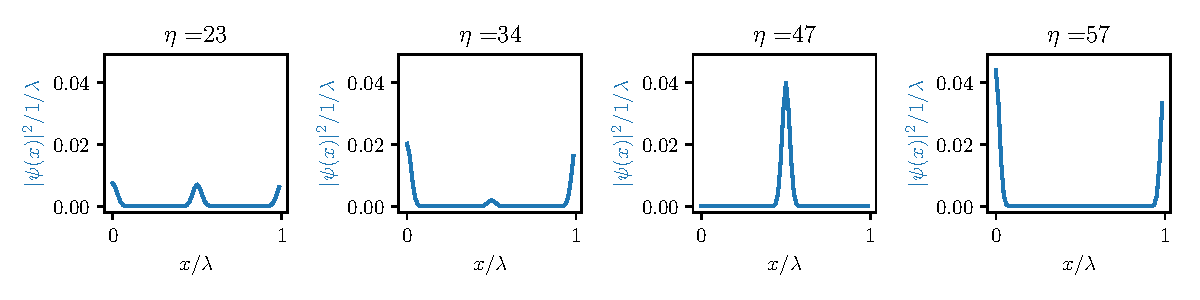
\includegraphics[width=1\textwidth]{images/model_limit_trans.pdf}
	\caption{Wave function densities as functions of $\eta$. At pumping strengths above $\eta = 23 \, \omega_\text{r}$, the periodicity changes and there are arbitrary positional jumps, thus putting the applicability higher pumping strengths into question.}
	\label{model_limit}
\end{figure}
\FloatBarrier
